%% Figure 1 (pgfplots). Data: results/paper/zero_readout_n16_8k (seeds 42-51, median and 25th-75th percentile band),
%% results/paper/fig2/n8_s42.json (target A_r) and results/paper/exact_spectra/sigma_sweep/s42_sg0.02.txt (Jacobian J_r).
\definecolor{stepc}{HTML}{0072B2}\definecolor{outc}{HTML}{D55E00}\definecolor{theoc}{HTML}{009E73}
\definecolor{modelc}{HTML}{7B4F9E}\definecolor{mutedc}{HTML}{6E6E6E}
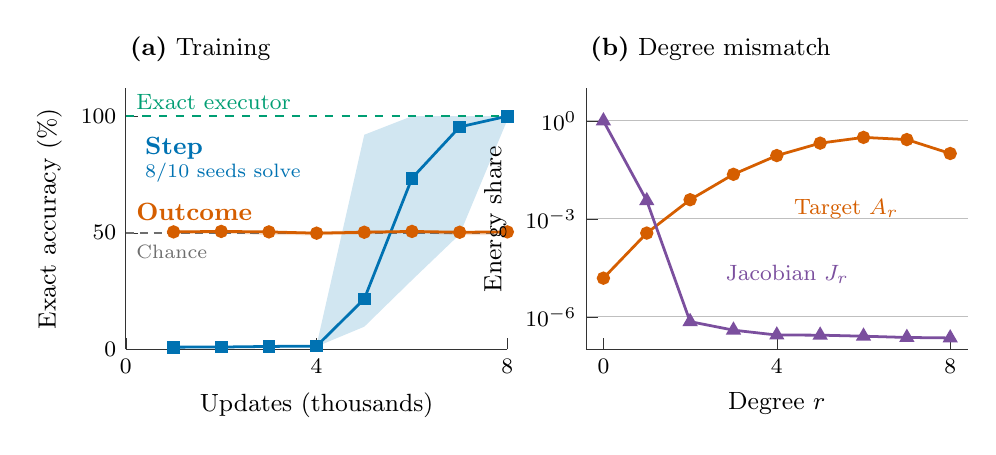
\begin{tikzpicture}
\pgfplotsset{every axis/.style={width=0.53\linewidth, height=4.9cm, axis line style={black!80}, tick style={black!80},
  tick label style={font=\footnotesize}, label style={font=\small}, title style={font=\small, at={(0,1)}, anchor=south west, xshift=-2pt}},
  every axis plot/.append style={line width=1pt}}
\begin{axis}[name=train, title={\textbf{(a)} Training}, xlabel={Updates (thousands)}, ylabel={Exact accuracy (\%)},
  xmin=0, xmax=8, ymin=0, ymax=112, xtick={0,4,8}, ytick={0,50,100}, axis x line*=bottom, axis y line*=left, clip=false]
  \addplot[draw=none, fill=stepc, fill opacity=0.18, forget plot] coordinates {(1,0.55) (2,0.73) (3,0.82) (4,1.25) (5,9.77) (6,29.75) (7,49.33) (8,98.40) (8,100.00) (7,100.00) (6,100.00) (5,92.03) (4,1.90) (3,1.40) (2,1.35) (1,1.35)};
  \addplot[draw=none, fill=outc, fill opacity=0.18, forget plot] coordinates {(1,49.52) (2,49.73) (3,49.05) (4,48.92) (5,49.35) (6,49.92) (7,48.97) (8,49.15) (8,50.70) (7,50.70) (6,51.20) (5,51.08) (4,50.60) (3,50.70) (2,51.08) (1,51.08)};
  \addplot[theoc, dashed, line width=0.9pt, domain=0:8, samples=2] {100};
  \addplot[mutedc, densely dashed, line width=0.8pt, domain=0:8, samples=2] {50};
  \addplot[stepc, mark=square*, mark size=1.8pt] coordinates {(1,1.00) (2,1.05) (3,1.30) (4,1.45) (5,21.65) (6,73.40) (7,95.40) (8,100.00)};
  \addplot[outc, mark=*, mark size=1.9pt] coordinates {(1,50.40) (2,50.60) (3,50.40) (4,49.85) (5,50.25) (6,50.60) (7,50.25) (8,50.40)};
  \node[anchor=south west, font=\footnotesize, text=theoc, inner sep=1pt] at (axis cs:0.15,101.5) {Exact executor};
  \node[anchor=west, font=\small\bfseries, text=stepc] at (axis cs:0.2,86) {Step};
  \node[anchor=west, font=\scriptsize, text=stepc] at (axis cs:0.2,76) {8/10 seeds solve};
  \node[anchor=south west, font=\small\bfseries, text=outc, inner sep=1pt] at (axis cs:0.15,54) {Outcome};
  \node[anchor=north west, font=\scriptsize, text=mutedc, inner sep=1pt] at (axis cs:0.15,46) {Chance};
\end{axis}
\begin{semilogyaxis}[at={(train.east)}, anchor=west, xshift=1.0cm, title={\textbf{(b)} Degree mismatch}, xlabel={Degree $r$},
  ylabel={Energy share}, xmin=-0.4, xmax=8.4, ymin=1e-7, ymax=10, xtick={0,4,8}, ytick={1e-6,1e-3,1},
  ymajorgrids, major grid style={black!25}, axis x line*=bottom, axis y line*=left]
  \addplot[outc, mark=*, mark size=1.9pt] coordinates {(0,1.5259e-05) (1,3.6621e-04) (2,3.8452e-03) (3,2.3071e-02) (4,8.6517e-02) (5,2.0764e-01) (6,3.1146e-01) (7,2.6697e-01) (8,1.0011e-01)};
  \addplot[modelc, mark=triangle*, mark size=2.2pt] coordinates {(0,9.9641e-01) (1,3.5840e-03) (2,7.1281e-07) (3,3.9081e-07) (4,2.7680e-07) (5,2.7450e-07) (6,2.5510e-07) (7,2.3310e-07) (8,2.2560e-07)};
  \node[anchor=north, font=\footnotesize, text=outc] at (axis cs:5.6,8e-3) {Target $A_r$};
  \node[anchor=west, font=\footnotesize, text=modelc] at (axis cs:2.6,2e-5) {Jacobian $J_r$};
\end{semilogyaxis}
\end{tikzpicture}
